\section{Date: 2026-09-28}
\noindent \textbf{Series ID: GLAKWPMANRGSP} 

\noindent This series is titled Real Gross Domestic Product: Wood Product Manufacturing (321) in the Great Lakes BEA Region and has a frequency of Annual. The units are Millions of Chained 2017 Dollars and the seasonal adjustment is Not Seasonally Adjusted.The observation start date is 1997-01-01 and the observation end date is 2024-01-01.The popularity of this series is 1. \\ 

\noindent \textbf{Series ID: ITCELSETSP2ECS} 

\noindent This series is titled Mobile Cellular Subscriptions: All Income Levels in Europe and Central Asia and has a frequency of Annual. The units are Number per 100 People and the seasonal adjustment is Not Seasonally Adjusted.The observation start date is 1960-01-01 and the observation end date is 2025-01-01.The popularity of this series is 1. \\ 

\subsection{Raw Regression}
\noindent Regresses the two series against each other directly. A significant result here can come just as easily from both series sharing a long-run trend as from any real relationship.

\begin{center}
\begin{tabular}{lclc}
\toprule
\textbf{Dep. Variable:}             & value\_fred\_ITCELSETSP2ECS & \textbf{  R-squared:         } &     0.083   \\
\textbf{Model:}                     &             OLS             & \textbf{  Adj. R-squared:    } &     0.048   \\
\textbf{Method:}                    &        Least Squares        & \textbf{  F-statistic:       } &     2.357   \\
\textbf{Date:}                      &       Mon, 28 Sep 2026      & \textbf{  Prob (F-statistic):} &    0.137    \\
\textbf{Time:}                      &           18:50:21          & \textbf{  Log-Likelihood:    } &   -142.11   \\
\textbf{No. Observations:}          &                28           & \textbf{  AIC:               } &     288.2   \\
\textbf{Df Residuals:}              &                26           & \textbf{  BIC:               } &     290.9   \\
\textbf{Df Model:}                  &                 1           & \textbf{                     } &             \\
\textbf{Covariance Type:}           &          nonrobust          & \textbf{                     } &             \\
\bottomrule
\end{tabular}
\begin{tabular}{lcccccc}
                                    & \textbf{coef} & \textbf{std err} & \textbf{t} & \textbf{P$> |$t$|$} & \textbf{[0.025} & \textbf{0.975]}  \\
\midrule
\textbf{const}                      &     285.3207  &      123.888     &     2.303  &         0.030        &       30.665    &      539.976     \\
\textbf{value\_fred\_GLAKWPMANRGSP} &      -0.0407  &        0.026     &    -1.535  &         0.137        &       -0.095    &        0.014     \\
\bottomrule
\end{tabular}
\begin{tabular}{lclc}
\textbf{Omnibus:}       &  3.492 & \textbf{  Durbin-Watson:     } &    0.174  \\
\textbf{Prob(Omnibus):} &  0.174 & \textbf{  Jarque-Bera (JB):  } &    2.983  \\
\textbf{Skew:}          & -0.713 & \textbf{  Prob(JB):          } &    0.225  \\
\textbf{Kurtosis:}      &  2.275 & \textbf{  Cond. No.          } & 7.63e+04  \\
\bottomrule
\end{tabular}
%\caption{OLS Regression Results}
\end{center}

Notes: \newline
 [1] Standard Errors assume that the covariance matrix of the errors is correctly specified. \newline
 [2] The condition number is large, 7.63e+04. This might indicate that there are \newline
 strong multicollinearity or other numerical problems.

\begin{figure}
\centering
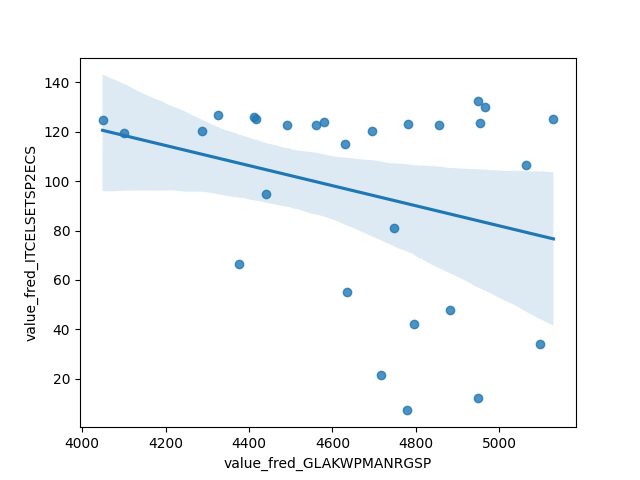
\includegraphics[scale = 0.9]{plots/plot_2026-09-28.png}
\caption{Raw Regression Plot for 2026-09-28}
\end{figure}
\newpage
\subsection{Detrended Regression}
\noindent Regresses the residuals of each series after removing its own linear time trend, so a shared trend can no longer drive the result on its own. A relationship that stays significant here is better evidence of a genuine link between the two series.

\begin{center}
\begin{tabular}{lclc}
\toprule
\textbf{Dep. Variable:}                        & value\_fred\_ITCELSETSP2ECS\_detrended & \textbf{  R-squared:         } &     0.184   \\
\textbf{Model:}                                &                  OLS                   & \textbf{  Adj. R-squared:    } &     0.152   \\
\textbf{Method:}                               &             Least Squares              & \textbf{  F-statistic:       } &     5.853   \\
\textbf{Date:}                                 &            Mon, 28 Sep 2026            & \textbf{  Prob (F-statistic):} &   0.0228    \\
\textbf{Time:}                                 &                18:50:21                & \textbf{  Log-Likelihood:    } &   -119.03   \\
\textbf{No. Observations:}                     &                     28                 & \textbf{  AIC:               } &     242.1   \\
\textbf{Df Residuals:}                         &                     26                 & \textbf{  BIC:               } &     244.7   \\
\textbf{Df Model:}                             &                      1                 & \textbf{                     } &             \\
\textbf{Covariance Type:}                      &               nonrobust                & \textbf{                     } &             \\
\bottomrule
\end{tabular}
\begin{tabular}{lcccccc}
                                               & \textbf{coef} & \textbf{std err} & \textbf{t} & \textbf{P$> |$t$|$} & \textbf{[0.025} & \textbf{0.975]}  \\
\midrule
\textbf{const}                                 &    1.116e-12  &        3.330     &  3.35e-13  &         1.000        &       -6.845    &        6.845     \\
\textbf{value\_fred\_GLAKWPMANRGSP\_detrended} &      -0.0283  &        0.012     &    -2.419  &         0.023        &       -0.052    &       -0.004     \\
\bottomrule
\end{tabular}
\begin{tabular}{lclc}
\textbf{Omnibus:}       &  0.861 & \textbf{  Durbin-Watson:     } &    0.444  \\
\textbf{Prob(Omnibus):} &  0.650 & \textbf{  Jarque-Bera (JB):  } &    0.837  \\
\textbf{Skew:}          &  0.216 & \textbf{  Prob(JB):          } &    0.658  \\
\textbf{Kurtosis:}      &  2.272 & \textbf{  Cond. No.          } &     285.  \\
\bottomrule
\end{tabular}
%\caption{OLS Regression Results}
\end{center}

Notes: \newline
 [1] Standard Errors assume that the covariance matrix of the errors is correctly specified.

\begin{figure}
\centering
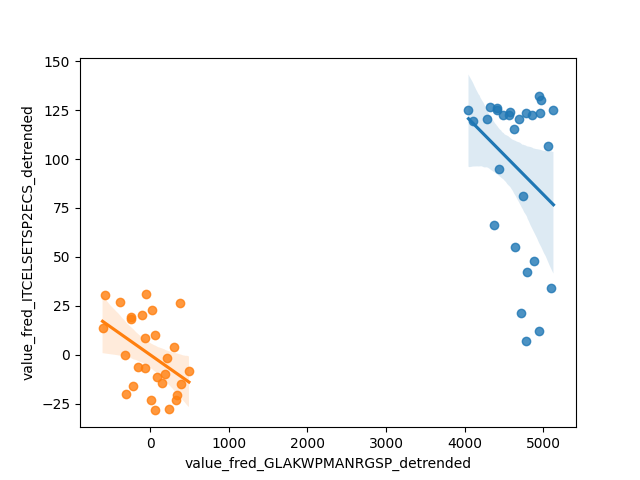
\includegraphics[scale = 0.9]{plots/plot_2026-09-28_detrended.png}
\caption{Detrended Regression Plot for 2026-09-28}
\end{figure}
\newpage
